\chapter{PP data analysis}
\label{chapter:analysis}
The HADES collaboration has performed a proton-proton experiment with beam kinetic energy 3.5 GeV in September 2012. Data collected during this experiment has allowed to conduct a series of analysis devoted to hyperons' studies \cite{hades_inclL_35,hades_L1405,hades_L1520,hades_PWA_pKpL,hades_S1385}. In the following thesis the hyperon studies is extended by a $\Ls$ inclusive reconstruction. A research conducted with a four particles $\p \pim \pip \pim$ final state allows to reconstruct the $\Ls X$ and  a $\Lz \Kz X$ inclusive signals. The obtained results were compared with a previous, exclusive measurements and used to constrain a simulation of a new experiment devoted to hyperon studies \ref{chapter:simulations}.

All methods developed for pp@3.5 GeV experiment were also used for data collected during pNb@3.5GeV experiment. The detailed description of the pNb data analysis is in Ch. \ref{chapter:analysis_pNb}. 

\section{Absolute normalization}
\label{sec:normalization}
An integrated luminosity for the pp experiment was calculated using a pp elastic scattering, measured in the same experiment \cite{hades_normalization}, it reached
\begin{equation}
  L^{int}=3.13 \cdot 10^8 mb^{-1}.
\end{equation}
Thanks to a full scale simulation performed in HYDRA framework (for more details see chapter \ref{chapter:simulations}) it is possible to simulate a detector response for every particles' combination end estimate how many of them could be properly reconstructed.  The efficiency, estimated by the simulation, together with the luminosity and a known \cs allows to determine expected count rates for any reaction.
\begin{equation}
  N^{\mathrm{expected}}_{pp\rightarrow X}=\frac{N_{\mathrm{reconstructed~in~simulation}}}{N_{\mathrm{simulated \; in \;} 4 \pi} \cdot 3} \cdot \sigma_{pp\rightarrow X} \cdot L^{int}.
\end{equation}
The factor 3 in denominator derives from the LVL1 trigger down-scaling. Due to limited read-out capabilities, for hadronic channels each 3th triggered event was saved on tapes. Thanks to the previous HADES research \cite{hades_inclL_35}, \css for many channels which can be a background source for $\Ls$ inclusive measurement. A list of all reactions simulated for following analysis is presented in tab. \ref{tab:channels}.  
\begin{table}
    \centering
  \caption{List of the channels considered in following chapter. All listed reaction can decay into a $\p \pim \pip \pim X$ final state, where X is an any particle. Starting from the  reaction no. 1 they are treated as a possible background channels. All values taken from \cite{hades_inclL_35}.}
  \label{tab:channels}
  \begin{tabular}{rll}
    \hline
    no. &Channel & $\sigma$ [$\mu \barn$]\\
    \hline
    \hline
    \multicolumn{3}{c}{3-body reactions} \\
    \hline
    0 & $\Ls \p \Kp$&$5.6 \pm 1.1 \pm 0.4 ^{+1.1} _{1.6}$\\
    1 & $\Lz \p \Kp$&$35.26 \pm 0.43 ^{+3.55}_{-2.83}$\\
    2 & $\Sz \p \Kp$&$16.5 \pm 20\%$\\
    3 & $\Lz \Dpp \Kz$&$29.45\pm 0.08 ^{+1.67}_{-1.46}\pm 2.06$\\
    4 & $\Sz \Dpp \Kz$&$9.26 \pm 0.05 ^{+1.41} _{0.31}\pm 0.65$\\
    5 & $\Sigma(1385)^+ \p \Kz$&$14.05 \pm 0.05 ^{+1.79}_{-2.14}\pm 1.00$\\
    6 & $\Dpp \Lss \Kz$&$5.0\pm 20\%$\\
    7 &$\Dpp \Ss \Kz$& $3.5 \pm 20\%$\\
    8 &$\Dp \Sigma(1358)^+ \Kz$&$2.3 \pm 20\%$\\
    \hline
    \multicolumn{3}{c}{4-body reactions} \\
    \hline
    9 &$\Lambda \p \pip \Kz $& $2.57 \pm 0.02 ^{+0.21}_{-1.98}\pm 0.18$\\
    10&$\Sz \p \pip \Kz$& $1.35 \pm 0.02 ^{+0.10}_{-1.35}\pm 0.09$\\
    \hline
  \end{tabular}
  
\end{table}

\section{Particles identification}
The HADES detector allows for two complementary methods of particles identification. The first, bases on particles' time of flight measured in the ToF detectors and particles' momentum measured in the MDC detector. These two quantities allows for a mass determination according to the formula
\begin{equation}
p=\gamma \beta m.  
\end{equation}
The second method, bases on the MDC exclusively and uses combine information about particles' momentum and energy losses ($\frac{dE}{dx}$) - both provided by MDC detector. These quantities are connected by the Boethe-Bolch formula:
\begin{equation}
  \frac{\mathrm{d}E}{\mathrm{d}x}=\frac{4 \pi N_A z^2 e^4}{mv^2} \frac{Z}{A} \left[ \ln \left(\frac {2mv^2}{I(1-\beta^2)} \right) - \beta^2 \right]
\end{equation}
which also allows to mark out a particle mass knowing a particle momentum and an energy loss.


In case of the HADES detector the first identification method is favoured, due to better precision, however a limited geometrical acceptance of the TOF detectors reduces detection efficiency by a factor 0.8 for each detected particle. In case of a four-particles final state, discussed in this thesis, a total loss caused by the TOF detectors can reach 60\% of all particles detected in the MDC. For that reason, the $\frac{de}{dx}$ vs. $\p$ method was used. Identification cuts have been optimized for previous analysis conducted by by HADES experiment and described in \cite{hades_inclL_35,lalik_phd}. Contours used for $\pim$ and $\pip$ are the same and differs only by electric charge, they are visualized in fig. \ref{fig:dedx}. 
\begin{figure}[h]
  \centering
  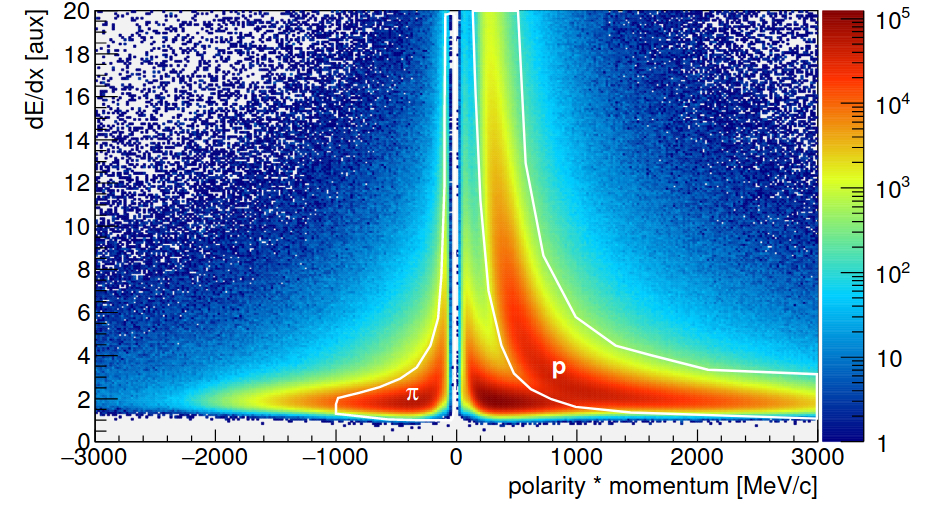
\includegraphics[width=0.9 \linewidth]{Chapter_analysis/DeDx_PPim.jpg}
  \caption{The identification cuts used in analysis. The contur for $\pip$ looks the same like for $pim$. Figure from \cite{hades_inclL_35}}
  \label{fig:dedx}
\end{figure}


\section{Event selection}
Among all registered events only these containing at least four charged particles (two positive and two negative) was considered in analysis. They have been also observed events with more than four particles detected (fig. \ref{fig:mult}). They produces combinatorics which are very difficult to control during further analysis. Because of that, only one four-particle combination from every event was considered in next steps. In every event all possible particles combinations were ordered according to track reconstruction quality. For each combination the sum of $\chi^2$ (match quality in MDCs) for all tracks was calculated, and the best reconstructed combination was taken. 

\begin{table}
  \centering
  \caption{An event selection steps}
  \label{tab:selection}
  \begin{tabular}{|c|c|}
    step & no. of hypothesis\\
    \hline
    \hline
    all 4-particle hypothesis& \\
    all hypothesis after de/dx cuts&6781970 \\
    hypothesis with the best $\chi^2$& 1917048\\
  \end{tabular}
\end{table}

Additionally an equivocation in $\pim$ selection requires some criteria to define which particle belongs to $\Lz$. In case on final spectrum $M^{inv}_{p \pim \pip \pim}$ a $\pim$ ordering make no difference, however for $\Lz$ reconstruction a different origin of two negative pions plays a crucial role. Fortunately a $\Lz$ hyperon is a very narrow resonance what gives a natural criteria for $\pim$ classification. Within one hypothesis, both $\pim$s were combined with a proton track and an invariant mass for those pairs ($\mathrm{M}^{inv}_{\p\pim}$) were calculated. The $\pim$ which gives better agreement with $\Lz$ pole mass (smaller $|M^{inv}_{p \pim} - M_{\Lz}|$) was treated as originated from secondary vertex.


\begin{figure}
  \centering
  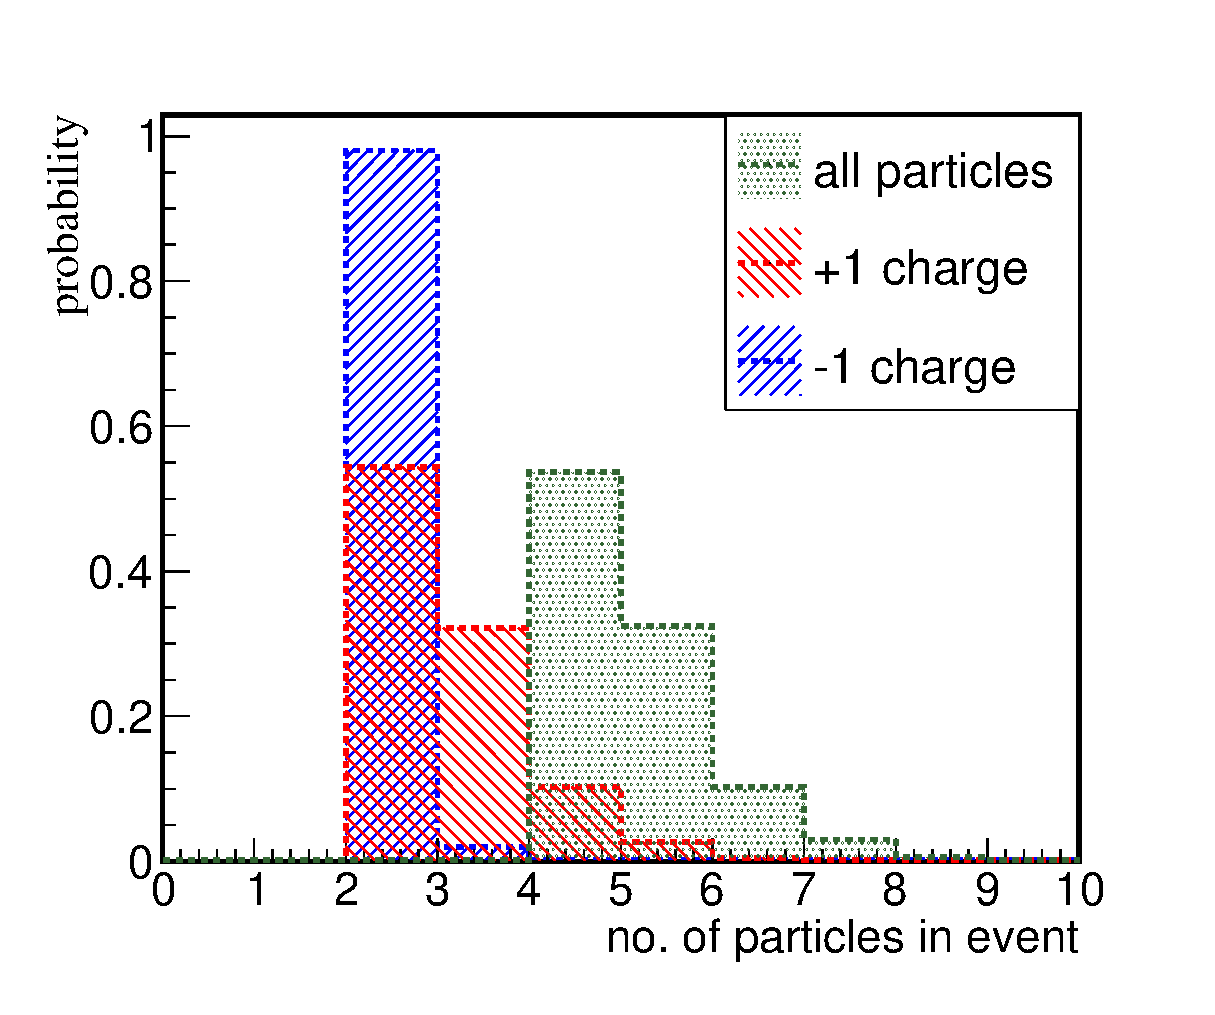
\includegraphics[width=0.7 \linewidth]{Chapter_analysis/mult.eps}
  \caption{Particles multiplicity for a final state which requires two particles witch charge +1 and two with -1. It is visible that only in 54\% cases exactly four charged particles, were registered by detector. All cases with more than 4 particles requires some criteria to take a proper combination from all possible. An asymmetry between positively- and negatively-charged particles is caused by an initial state electric charge. Particles identification was done based on de/dx cuts.}   
  \label{fig:mult}
\end{figure}



\section{Reaction kinematics}
\label{section:kinematics}
For pp@3.5 GeV collisions the production threshold for $\Ls$ ($\sqrt{S_{E_K=3.5GeV}}-E^{\mathrm{thr}}_{\p\Kp\Ls}=0.22 GeV$) lies just below available energy threshold.  Using the rule of a energy-momentum conservation is possible to calculate missing mass for observed particles. Because of small excess energy, which does not allow for others particles creation, a dominant, and probably only one, channel for $\Ls$ production is as follows
\begin{equation}
  \p\p \rightarrow \p \Kp \Ls [\Lz \pip \pim].
\end{equation}
In this reaction the smallest missing mass for the $\p \pim \pip \pim$ final state is $\Sqs - \Ls_{mass}= 1432$ MeV. It is a very strong kinematic constrain, which separates well the signal from most of background channels. The missing mass spectrum is presented in fig. \ref{fig:missMass}. There is visible a resonance behaviour around 1200 MeV. Due to conservation rules missing particles have to have a total charge +2 and a baryon number +1. It leads to the conclusion that the missing mass spectrum is dominated by a $\Dpp$ production. Indeed a simulation confirmed that peak around 1200 MeV originates from $\Dpp$ decaying into $\p \pip$. A mass shift and signal shape are caused by protons mismatch. In reaction
\begin{equation}
  \label{eq:dpp}
  \p\p \rightarrow \Dpp [\p \pip] \p \pim \pim \pip
\end{equation}
both protons can be combined with $\pip$. The selection procedure, describe in the section above, protect against double-counting and wrong $\pim$ assignment, but do not provide faultless $\Dpp$ reconstructions. It leads to mixing between protons and pions and a $\Dpp$ spectrum distortion. A \ref{eq:dpp} was simulated and reconstructed using full analysis chain. Results are shown in \ref{fig:missMass}.

\begin{figure}[ht]
  \centering
  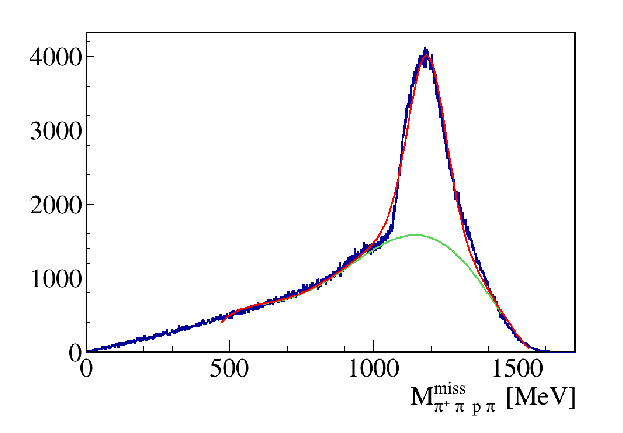
\includegraphics[width=0.9 \linewidth]{Chapter_analysis/missMass.eps}
  \caption{The missing mass of $\p \pim \pip \pim$ system for an experimental data (blue line) and simulations. The resonance behaviour around 1200 MeV is clearly visible. The magenta histogram represents perfectly reconstructed $\Dpp$ from the background channel $\p\p \rightarrow \Dpp [\p \pip] \p \pim \pim \pip$. The green histogram shows input from this channel reconstructed by analysis algorithm designed for $\Ls$ reconstruction. An inconsistency between the perfect and the real reconstruction is described in text. Both simulation histograms were arbitrary scaled up to have the same high like data.}
  \label{fig:missMass}
\end{figure}


Because in the  energy regime almost all pions are produced via barionic resonances, and $\Dpp$s tend to be produced in pairs, it was expected that an invariant mass of $\p \pip$ detected in experiment would also contain a strong $\Dpp$ component. Indeed, as it is shown in fig. \ref{fig:dpp2D} most of the background comes from correlated source with maximum yield around double $\Dpp$ production. The figure shows also that a cut on missing mass > 1432 MeV removes a significant part of a background events.

Except an inclusive $\Ls$ reconstruction the final state $\Lz \pip \pim$ may be used for $\Lz \Kz X$ reconstruction. In this case (see. \ref{section:LzKz}) the missing mass cut was different due to different overall kinematics.  The cat put on a mass $M^{miss}_{\p \pip \pip \pim}>1077$, what is the smallest missing mass required in
\begin{equation}
\p\p \rightarrow \Lz \Kz \p \pip
\end{equation}
reaction. Unfortunately lower value for the $M^{miss}$ cut effects a data sample contamination by $\Dpp$ decays, what is clearly visible in \ref{fig:dpp2D}. 


\begin{figure}[ht]
  \centering
  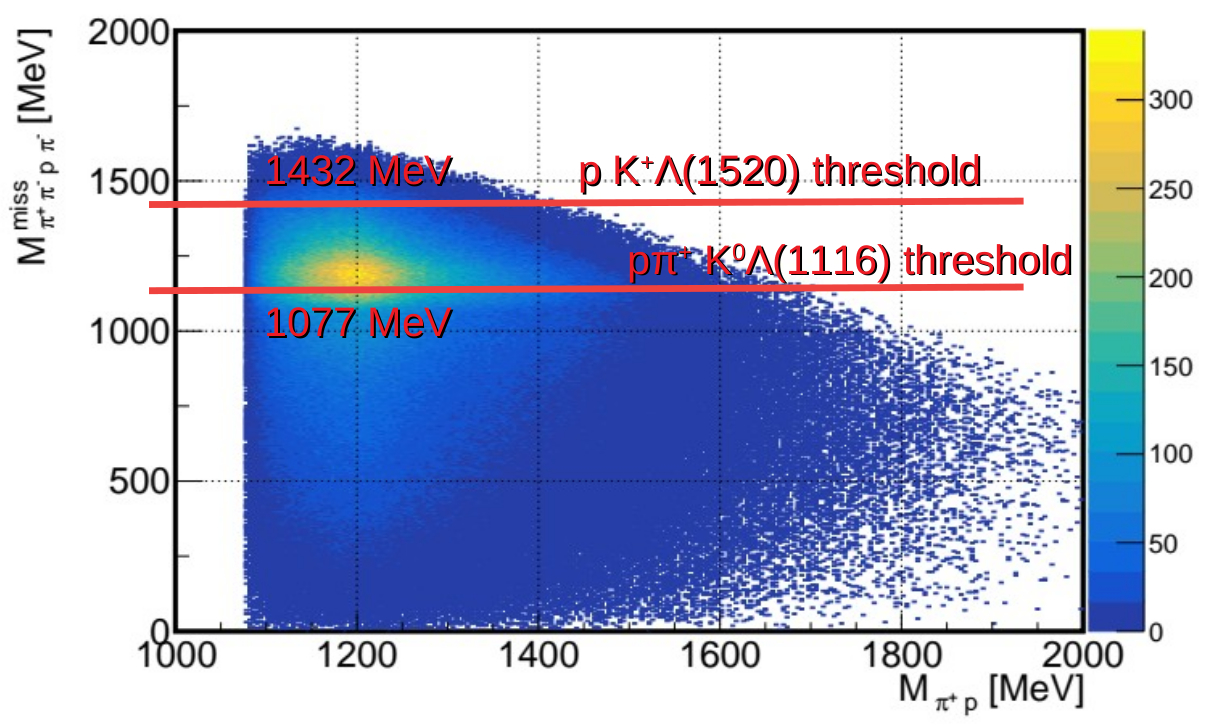
\includegraphics[width=0.9 \linewidth]{Chapter_analysis/Miss_PPip.jpg}
  \caption{The missing mass of $\p \pim \pip \pim$ system vs. invariant mass of a $\p\pim$ system. It is clearly visible that most of the background comes from correlated source of two $\Dpp$ production. Such situation helps to easy discriminate most of the background. Two red horizontal lines denotes minimal missing mass required for $\Ls$ and $\Lz$ production for $\p \pim \pip \pim$ final state.}
  \label{fig:dpp2D}
\end{figure}

\section{The $\Lz$ Reconstruction}
The next step of the analysis after a missing mass cut was an inclusive $\Lz$ reconstruction. In previous HADES experiments the reconstruction had based on a set of geometrical cuts. Their role was to increase a signal-to-background ratio, utilizing a $\Lz$ decay geometry. The $\Lz$ resonance decays via week interactions, so its lifetime is relatively long: $c\tau = 7.89 \mathrm{cm}$ \cite{PDG}. That may be used to discriminate an out of target $\Lz$'s decay vertex, from a background originates from strongly decaying non-strange barionic resonances.

\begin{figure}[h]
  \centering
  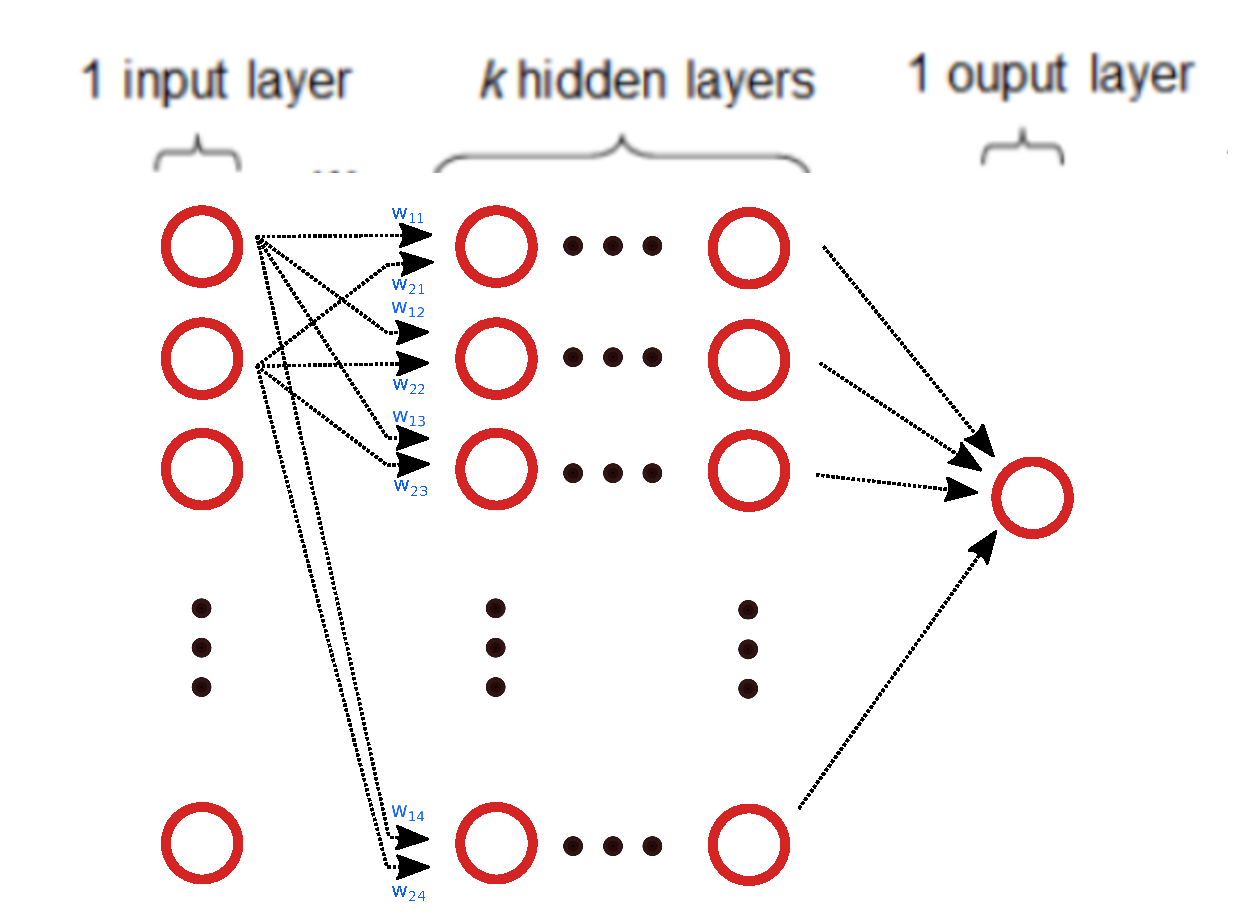
\includegraphics[width=0.7 \linewidth]{Chapter_analysis/NN.eps}
  \caption{An architecture of a neural network used in analysis. For a simplicity only connections of the first neuron from the first layer were drawn. In dense network output from each of neurons is passed to every neuron in a next layer. A particular designed used for a $\Lz$ reconstruction consist of 4 layers: an input layer and 3 hidden layers. The network width (number of neurons in one layer) was adjusted to amount of input parameters and was 20.}
  \label{fig:NN}
\end{figure}

As it was shown in \ref{section:kinematics} an available phase-space for $\Ls$ production for a $E_k=3.5$ GeV is very limited. An inclusive analysis performed in \cite{hades_L1520} has measured  $\Ls$, however an yeld reached only ??? events. To improve the signal yield, and also examine new reconstruction methods, in following analysis a neural network was used as a replacement of the geometrical cuts. Details about used method and an optimization process are explained in chapter \ref{chapter:NN}.

\begin{figure}[h]
  \centering
  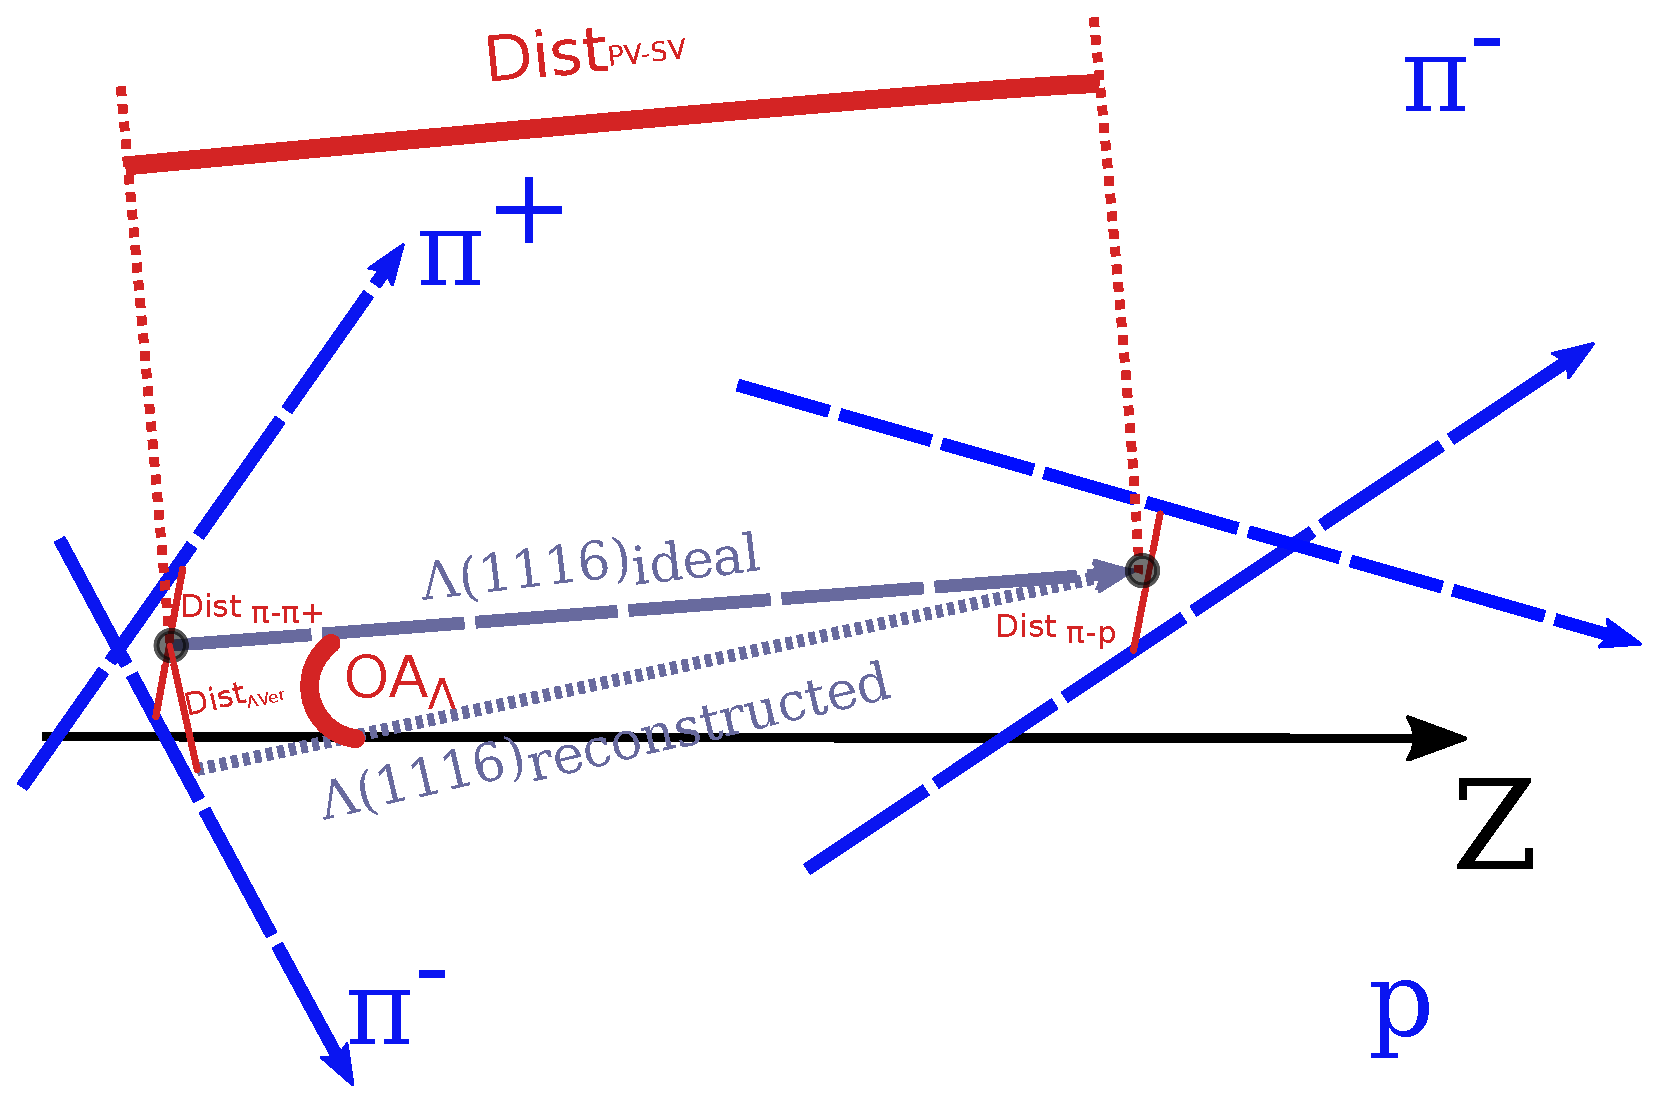
\includegraphics[width=0.7 \linewidth]{Chapter_analysis/geometria_NN.eps}
  \caption{A graphical representation of variables used as an input for neural network.}
  \label{fig:NN_cuts}
\end{figure}


The final network architecture used for $\Lz$ reconstruction is a feed-forward, dense network, consist of 4 layers, each N+6 neurons, where N is a number of scalar input parameters. For each neuron a sigmoid was used as an activation function. Because the network replaced geometrical cuts, eleven geometrical variables had been taken as the network's input:

\begin{itemize}
\item Distance between $\p \pim$ from $\Lz$
\item Distance between $\pip$ and $\pim$ from primary vertex
\item $\Lz$ vertex coordinates, reconstructed as a point of the closest approach of $\p$ and $\pim$ tracks
\item $\Ls$ vertex coordinates, reconstructed as a point of the closest approach of $\pip$ and $\pim$ tracks
\item $\Ls$ vertex coordinates, reconstructed by tracking algorithm as a primary vertex
\item Opening angle between reconstructed $\Lz$ vector and a line connecting primary and secondary vertices
\item Distance between $\p$ from $\Lz$ decay and primary vertex
\item Distance between $\pim$ from $\Lz$ decay and primary vertex
\item Distance between reconstructed $\Lz$ direction and primary vertex
\item Distance between primary and secondary vertexes
\end{itemize}

Additionally the chosen parameters do not allow for $\Lz$ invariant mass reconstruction. That was crucial to learn the network geometrical properties not just invariant mass reconstruction, otherwise the network would replace a $\p \pim$ invariant mass cut, instead of cuts on geometrical properties. That may be understood as a network tendency to recognize the most significant discriminant in a data set. Because $\Lz$ is narrow the easiest way to increase signal to background ratio is reject all events with $M^{inv}_{\p \pim}$ different than $\Lz$ mass, but it would not be the network goal.

The optimized neural network may enhanced a signal to background ratio from 0.345 without any cuts to 16 for very restricted cut. However with increasing S/B ratio a final statistics was reduces as well. The final cut was optimized to get the best $\Ls$ signal, not $\Lz$. After an optimization the cut was set 0.59 and obtained $\Lz$ signal is shown in fig \ref{fig:L1116SB}. The signal to background ratio is ???, but all uncorrelated background can be removed by a side-band method. The signal obtained in this way was used for a next steps of analysis: the $\Ls$ analysis (chapter \ref{section:Ls}) and associated $\Lz \Kz$ production (chapter \ref{section:LzKz});

\begin{figure}[h]
  \centering
  %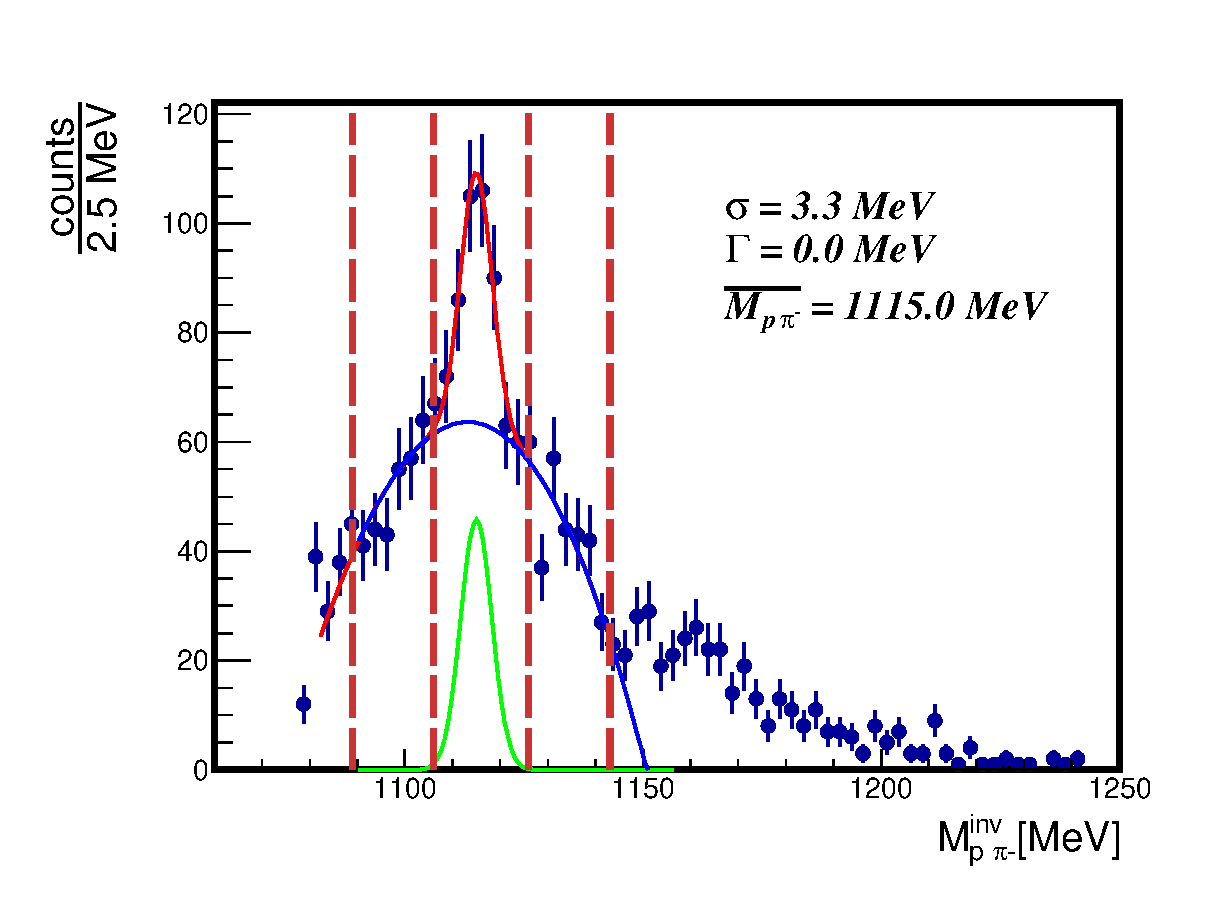
\includegraphics[width=0.7 \linewidth]{Chapter_analysis/L1116SB.eps}
  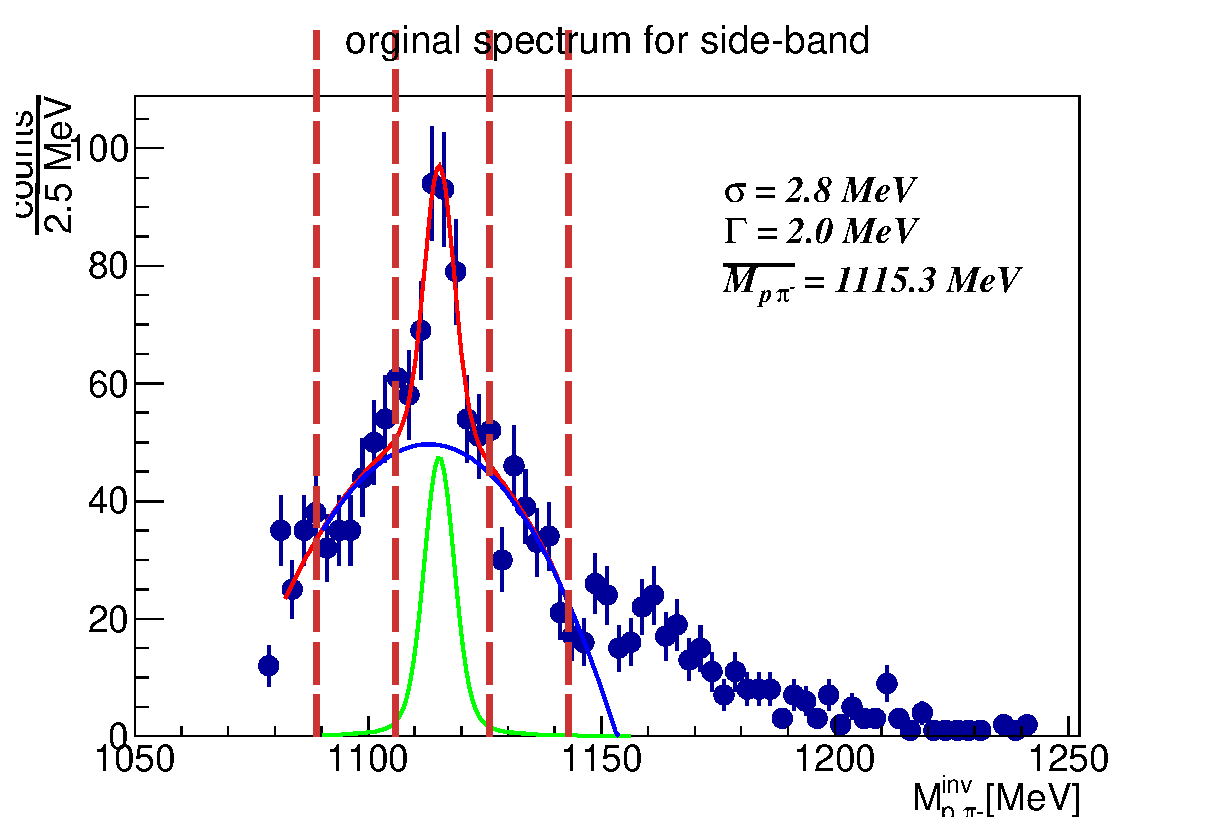
\includegraphics[width=0.7 \linewidth]{Data_pp/canvas_cSB.eps}
  \caption{The $\Lz$ spectrum after a neural network analysis. The vertical lines denotes regions of a side-band analysis described in \ref{section:SB}. The data was fitted by a sum of 4-th order polynomial (blue line) and a Voigt function (green line. A very small value for $\Gamma$ parameter is caused by the $\Lz$ long live-time. Obtained $\sigma$ value describe an apparatus energy resolution. }
  \label{fig:L1116SB}
\end{figure}


\section{The $\Lz \Kz $reconstruction - a reference channel}
\label{section:LzKz}
Due to the strangeness conservation law a $\Lz$ has to be produced with some anti-strange particle. The lightest candidate is a $\Kz$ meson, which decays in 69.2\% into $\pip \pim$ pair \cite{PDG}. For that reason a $\Lz \Kz$ signal is expected to be a significant part of the $\Lz \pip \pim$ final state and should be visible in analyzed data. Almost whole contamination from $\Kz$ decay may be removed by a cut on $M^{inv}_{\pip \pim}<410 \mathrm{MeV}$ without the signal affection. However a semi-inclusive $\Lz \Kz$ production may be a good reference channel for the analysis.

Because a kinematics for a $\Lz \Kz$ production is different than for $\Ls$, the used missing mass cut was looser than in $\Ls$ analysis. It was set  $M^{miss}_{\p \pip \pip \pim}>1077$, what is a minimal missing mass expected for $pp \rightarrow p \Kz \Lz \pip$ reaction with $\p_{E_k}=3.5 \mathrm{GeV}$. A $\Lz$ reconstruction, performed by neural networks, was the same as for the signal channel wieth the same cut value.

After the $\Lz$ reconstruction two spectra were drown: a) a $M^{inv}_{\pip \pim}$ invariant mass spectrum for events in $\Lz$ mass range ($1006<M^{inv}_{\p \pim}<1026$) and b) a $\mathrm{M}^{inv}_{\p\pim}$ invariant mass for $480 MeV< \mathrm{M}^{inv}_{\pip \pim}<500 MeV$. Obtained spectra had to be compared with simulation, so the same analysis chain was used to analyzed all channels listed in \ref{tab:channels} which contains associated $\Lz\Kz$ production (no 3-10). Summing up all \css for exclusive channels, the total inclusive $\Lz \Kz$ \cs $\approx 68 \mathrm{\mu b}$ was obtained.

In a given energy range a major part of a pion production proceeds by a resonance decays. A lack of reliable production models, especially for $\Dpp$ production and decay, do not allow for an exact simulation. Thence all background channels were simulated with the same kinematics of a $\p\p \rightarrow \p \Lz \Kz \pip$ reaction. Using a procedure described in \ref{sec:normalization} the simulation was compared with experimental data (see \ref{fig:K0L0}). The simulation describes reasonable well a yield of $\Kz$ and $\Lz$ produced in experiment, although it does not describe the background shape. This is mostly caused by lack of reliable model for a double $\Dpp$ production and decay. 

\begin{figure}[th]
  \centering
  % 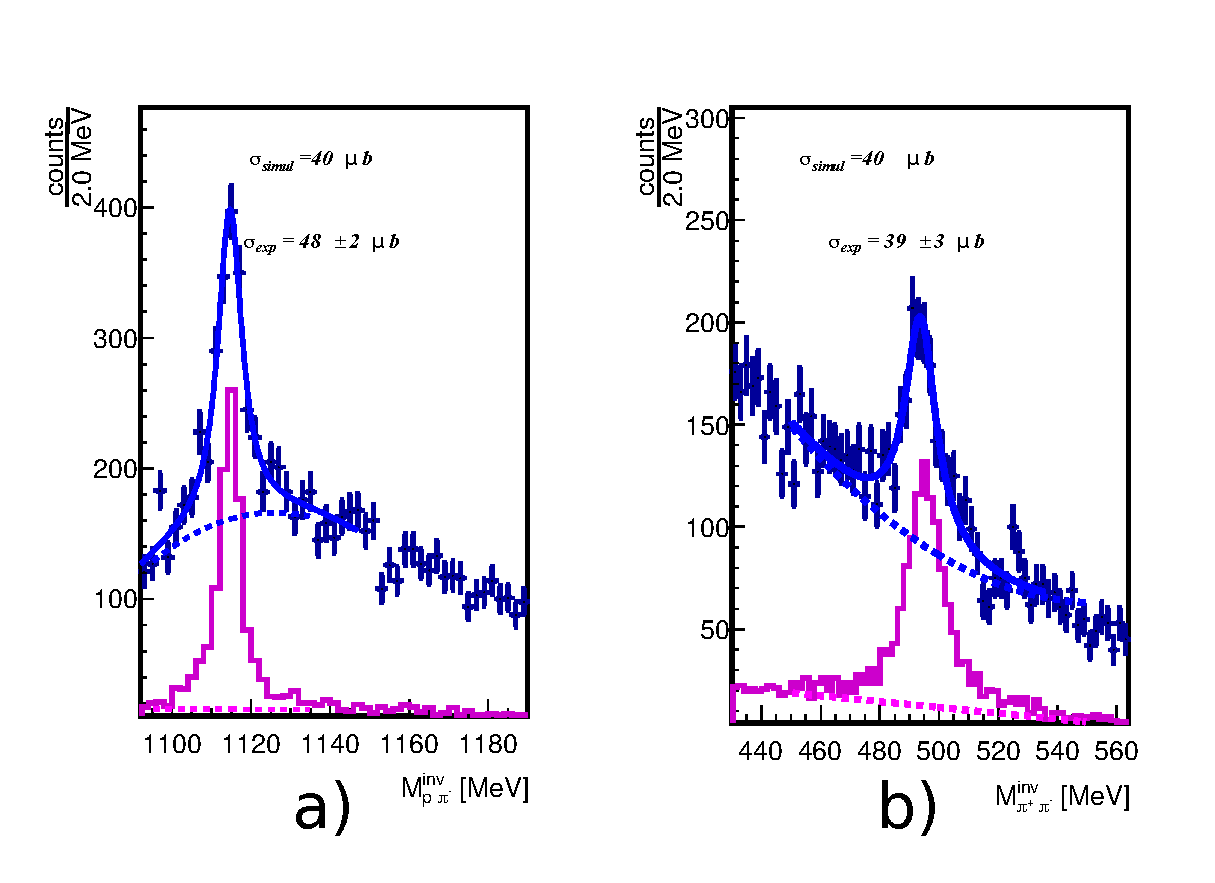
\includegraphics[width=1.1 \linewidth]{Chapter_analysis/K0L0_indeksy.eps}
  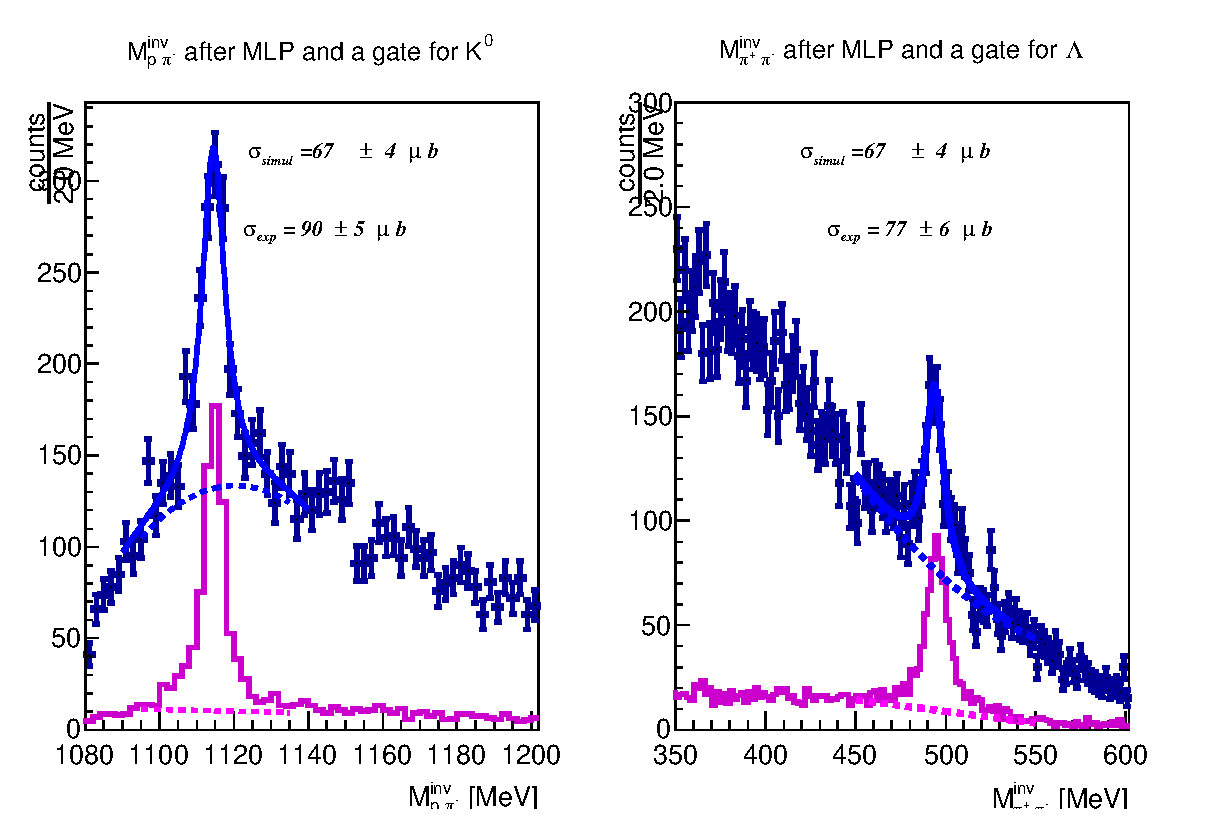
\includegraphics[width=1.1 \linewidth]{Data_pp/canvas_cLK0.eps}
  \caption{The results for $\Lz \Kz$ associated production. Blue point represents experimental data, magenta a sum simulated channels. For both: the simulation and the experimental data a Voigt function was fitted. Than, a total signal yield between simulation and experiment was calculated. The reconstruction efficiency was estimated base on $\p\p \rightarrow \Lz\Kz\p\pip$ reaction.}
  \label{fig:K0L0}
\end{figure}



\section{The $\Ls$ Reconstruction}
\label{section:Ls}
The neural network analysis gives a data sample with good S/B ratio for $\Lz$ signal. However set of additional cuts has to be applied to extract a $\Ls$ signal from the data. Using the signal channel's simulation a set of hard cuts was optimized: i) a distance between a secondary vertex (SV) and a primary vertex (PV) has to be larger than 5 mm, ii) an opening angle ($\mathrm{OA}_\Lz$) between a reconstructed $\Lz$ momentum direction and line connecting the primary and secondary vertexes has to be smaller than 20 degree . The cuts are illustrated in fig. \ref{fig:Ls_cuts}. A $p \pim \pip \pim$ spectrum obtained after the hard cuts contain both: a $\Ls$ signal and background originated from background under a $\Lz$ peak. To remove that contamination an additional steps were necessary. One of them was a side-band analysis which allowed to remove uncorrelated combinatorial background from $\Ls$ spectrum.
\begin{figure}[hb]
  \centering
  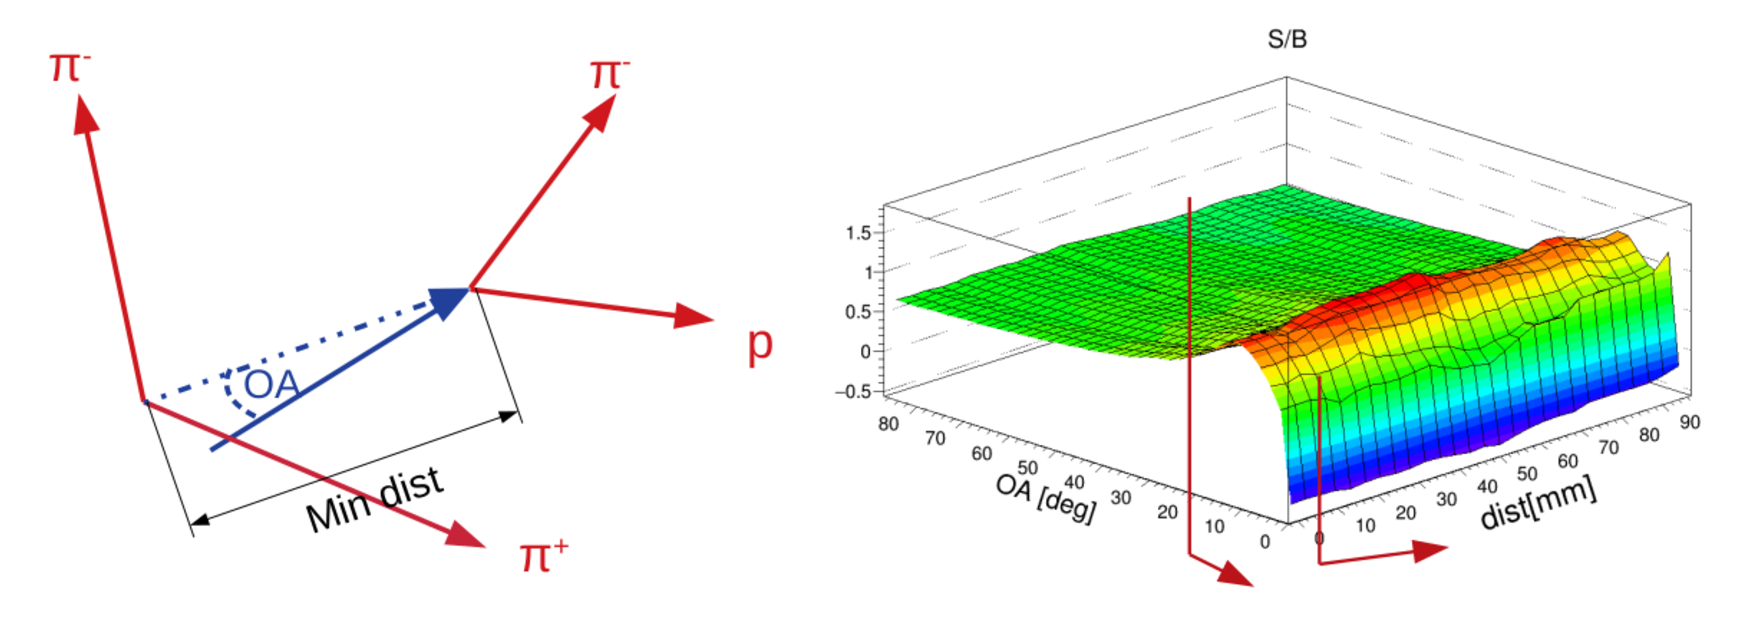
\includegraphics[width=0.9 \linewidth]{Chapter_analysis/HC_optymalizacja.eps}
  \caption{Cuts used for a $\Ls$ reconstruction. They were optimized using simulation of a signal channel $\p\p \rightarrow \Ls[\Lz \pip \pim] \p \Kz$. Lack of background channel is visible in constant S/B ratio for distance between primary and secondary vertex. For that reason A cut was set on 5 mm - it rejects most of decays inside the target.}
  \label{fig:Ls_cuts}
\end{figure}



\subsection{Side-band analysis}
\label{section:SB}
A side-band analysis bases on an assumption that kinematics of a background events changes slowly through a spectrum. Thanks to this, kinematics of the background events from signal region can be well described by background events from close neighbourhood of the signal region. In case of described analysis the side-band method was used to estimate an impact of non-perfect $\Lz$ reconstruction for the $\Ls$ spectrum.

The fig. \ref{fig:L1116SB} shows input for the side-band. The spectrum is divided by red dashed lines into three sections. The middle one is a signal range, the left and  the right are side-band regions. A corresponding $M^{inv}_{p \pim \pip \pim}$ spectra are shown in \ref{fig:Ls_SB}. Blue line shows signal after $\Lz$ reconstruction, the opening angle and the PV-SV distance cuts, for $M^{inv}_{\p \pim}$ in $\Lz$ range. The red points shows the $M^{inv}_{p \pim \pip \pim}$ from SB regions. The side-band describes very well both wings of the data distribution. A difference between signal and the side-band spectrum can be interpreted as $\p \pim \pip \pim$ signal associated exclusively with the $\Lz$ signal.
\begin{figure}[h]
  \centering
  % 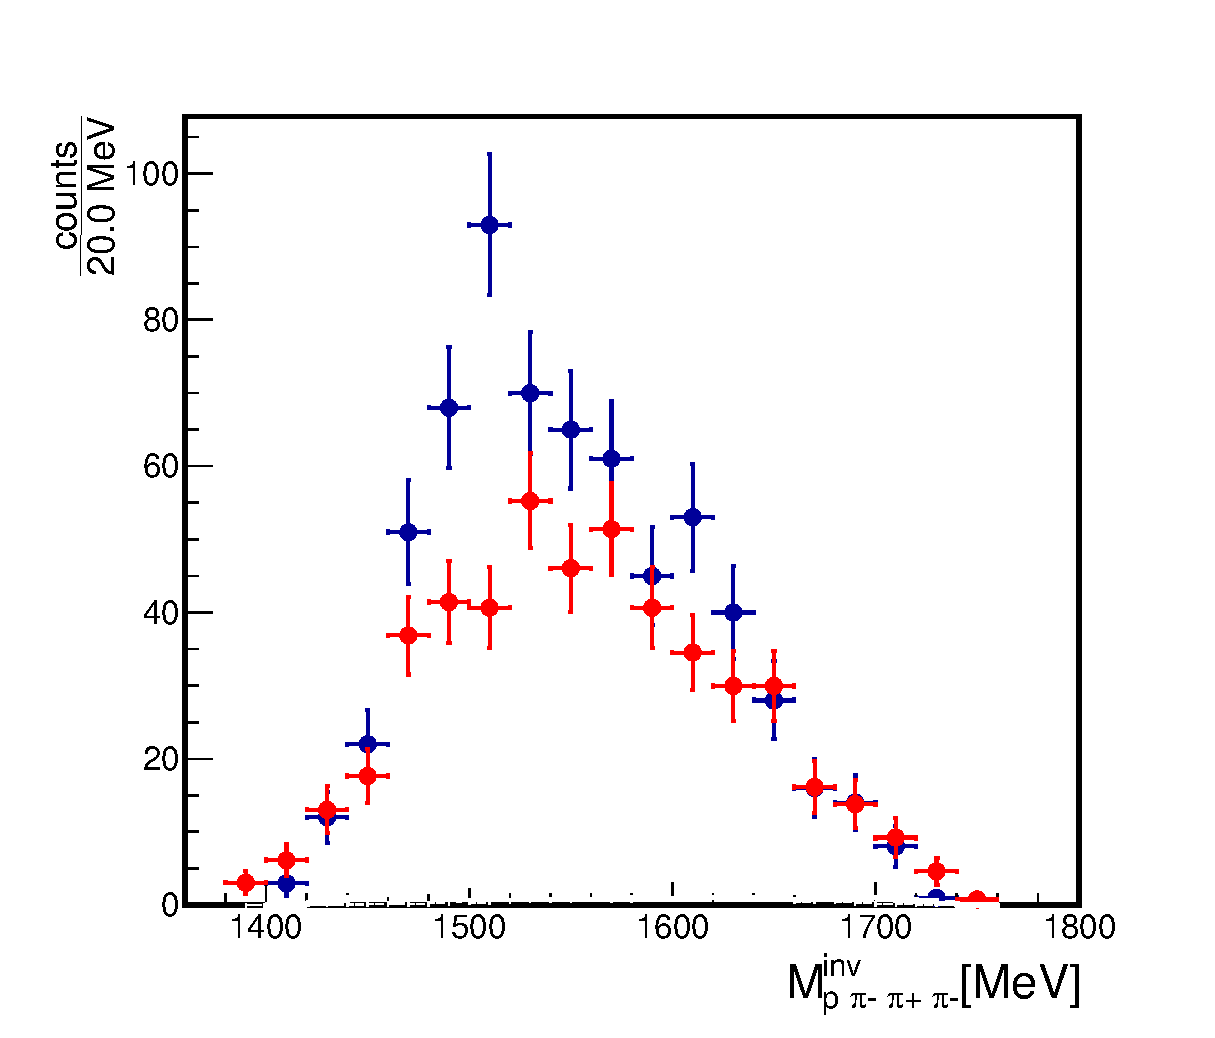
\includegraphics[width=0.7 \linewidth]{Chapter_analysis/L1520_sig_SB.eps}
  \includegraphics[width=0.7 \linewidth]{Data_pp/canvas_cSum_thesis.eps}
  \caption{The $M^{inv}_{\p \pim \pip \pim}$ spectrum for events from signal region ($M_{\p \pim}^{inv}\in(1106,1126)$) -blue points, and from SB regions ($M_{\p \pim}^{inv}\in(1089,1106] \cup [1126,1143)$) - red points. The SB spectrum was normalized to the background area from fig. \ref{fig:L1116SB}. Error bars shows a statistical uncertainty.}
  \label{fig:Ls_SB}
\end{figure}

\subsection{Cross-section extraction and differential analysis}
The side-band analysis has shown that for the $M^{inv}_{\p\pim\pip\pim}$ spectrum in an area between 1460 and 1600 MeV there is a signal corelated with $\Lz$ production. It is better visible after a SB substruction in \ref{fig:Ls_clean} b). A big statistical errors follows a substruction of two histograms: the signal and the SB.

Despite the side-band spectrum describes an uncorelated background's shape very well, there is still visible some signal contamination in a mass region over 1540 MeV , see fig. \ref{fig:Ls_clean}. It may be caused by correlated combinatorial background, when corelated $\pip \pim$ pair is combined with real $\Lz$ signal. The main source of di-pion pairs, a $\Kz$ decay, is suppressed by a cut $M^{inv}_{\pip \pim}<410 MeV$. However there are reactions which allows for mixing pions from two different sources. Three of them were chosen as the most important ones. They are presented in tab. \ref{tab:channels} with numbers 3-5. the final state for each of them contains $\Lz$ and two different sources of pions. An combination of a $\pim$ from a $\Kz$ decay and a $\pip$ from a $\Dpp$ or a $\mathrm{\Sigma^+}$ creates an correlated combinatorial background associated with the real $\Lz$ signal. 

\begin{figure}[h]
  \centering
  % 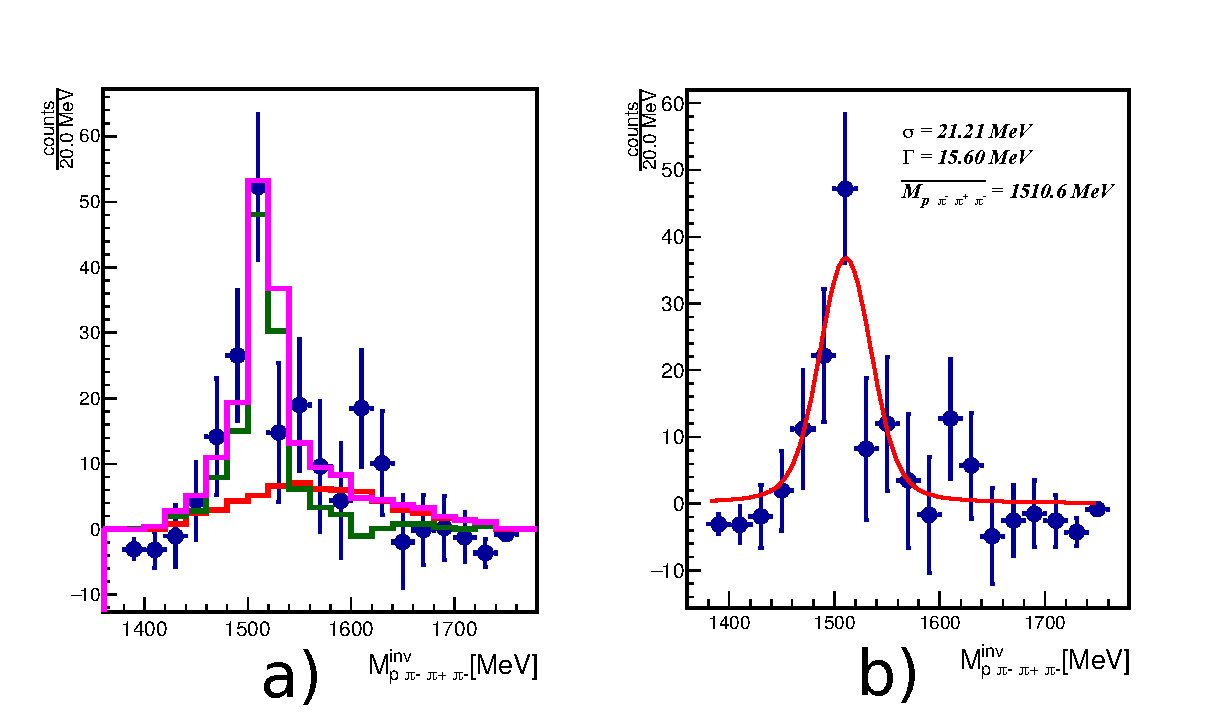
\includegraphics[width=0.9 \linewidth]{Chapter_analysis/L1520_sig_Clean.eps}
  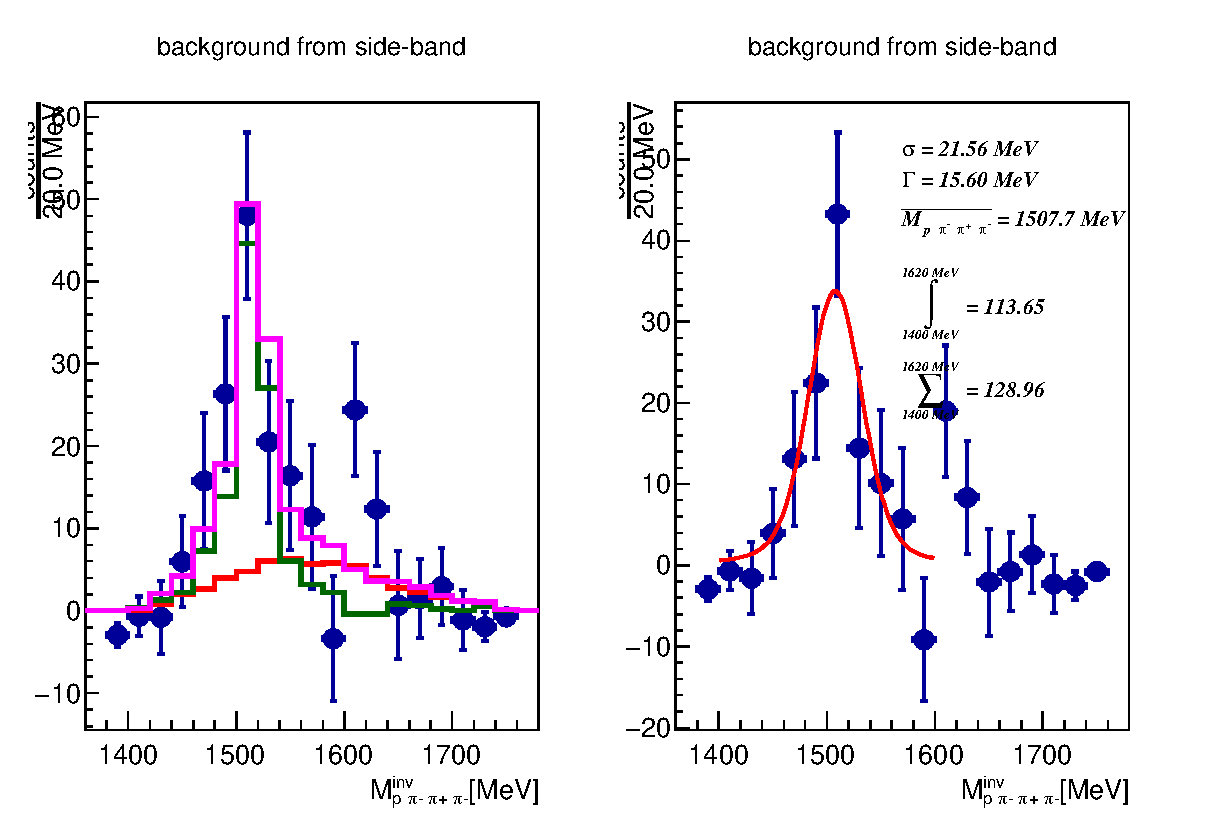
\includegraphics[width=0.9 \linewidth]{Data_pp/canvas_cClean_ren.eps}
  \caption{The $\Ls$ signal obtained in experiment. a) The experimental spectrum after a side-band subtraction (blue points) together with the signal and the background simulation (green and red line respectively). The magenta line shows the sum of all simulated channels. b) Signal after the simulated background subtraction. The Voigt functions used to describe the data points was constrained by a known $\Ls$ decay width $\Gamma=15.6 \mathrm{MeV}$ \cite{PDG}. Obtained $\sigma$ value can be treated as a measure of energy resolution obtained in the experiment. A shift of a pole mass is coused by a particles energy losses in MDC, wich hadn't been corrected during reconstruction.}
  \label{fig:Ls_clean}
\end{figure}

An identification of the background channels allows to simulate them and evaluate the corelated signal contamination. The signal channel was simulated according to exclusive cross section measured by HADES $\sigma_{\p\p\rightarrow \p \Kp \Ls}=6.5 \mathrm{\mu b}$ \cite{hades_L1520}. The signal and the backgroud channels were added together and compared with experimental result. Because a result was systematiclly below data points, the simulated signal spectrum was scaled up to get the same area under the total simulation spectrum and the experimental histogram. Finally, according to the obtained scaling an inclusive \cs is equal $\sigma_{\p\p \rightarrow \Ls \mathrm{X}}=9.1\pm 1.7 \mathrm{\mu b}$. An uncertainty comes from a statistical error. The signal enchancement visible in right part of the spectra, around 1650 MeV, can not be explained in simple way. It is also visible in data from exclusive $\Ls$ analysis \cite{hades_L1520} and stay still as an open question.



The total yield of detected decays allows to conduct a simple differential analysis. For events from a $\Ls$ mass range ($M^{inv}_{\p\pim\pip\pim} \in (1440 \mathrm{MeV}, 1600 \mathrm{MeV})$) transverse momentum ($p_t$) and a rapidity ($\Upsilon$) was calculated. Obtained spectra are presented in fig. \ref{fig:WPt}. The simulation reconstructs a general trend in distributions, however a limited statistics do not allow for more conclusive results.
\begin{figure}[h]
  \centering
  %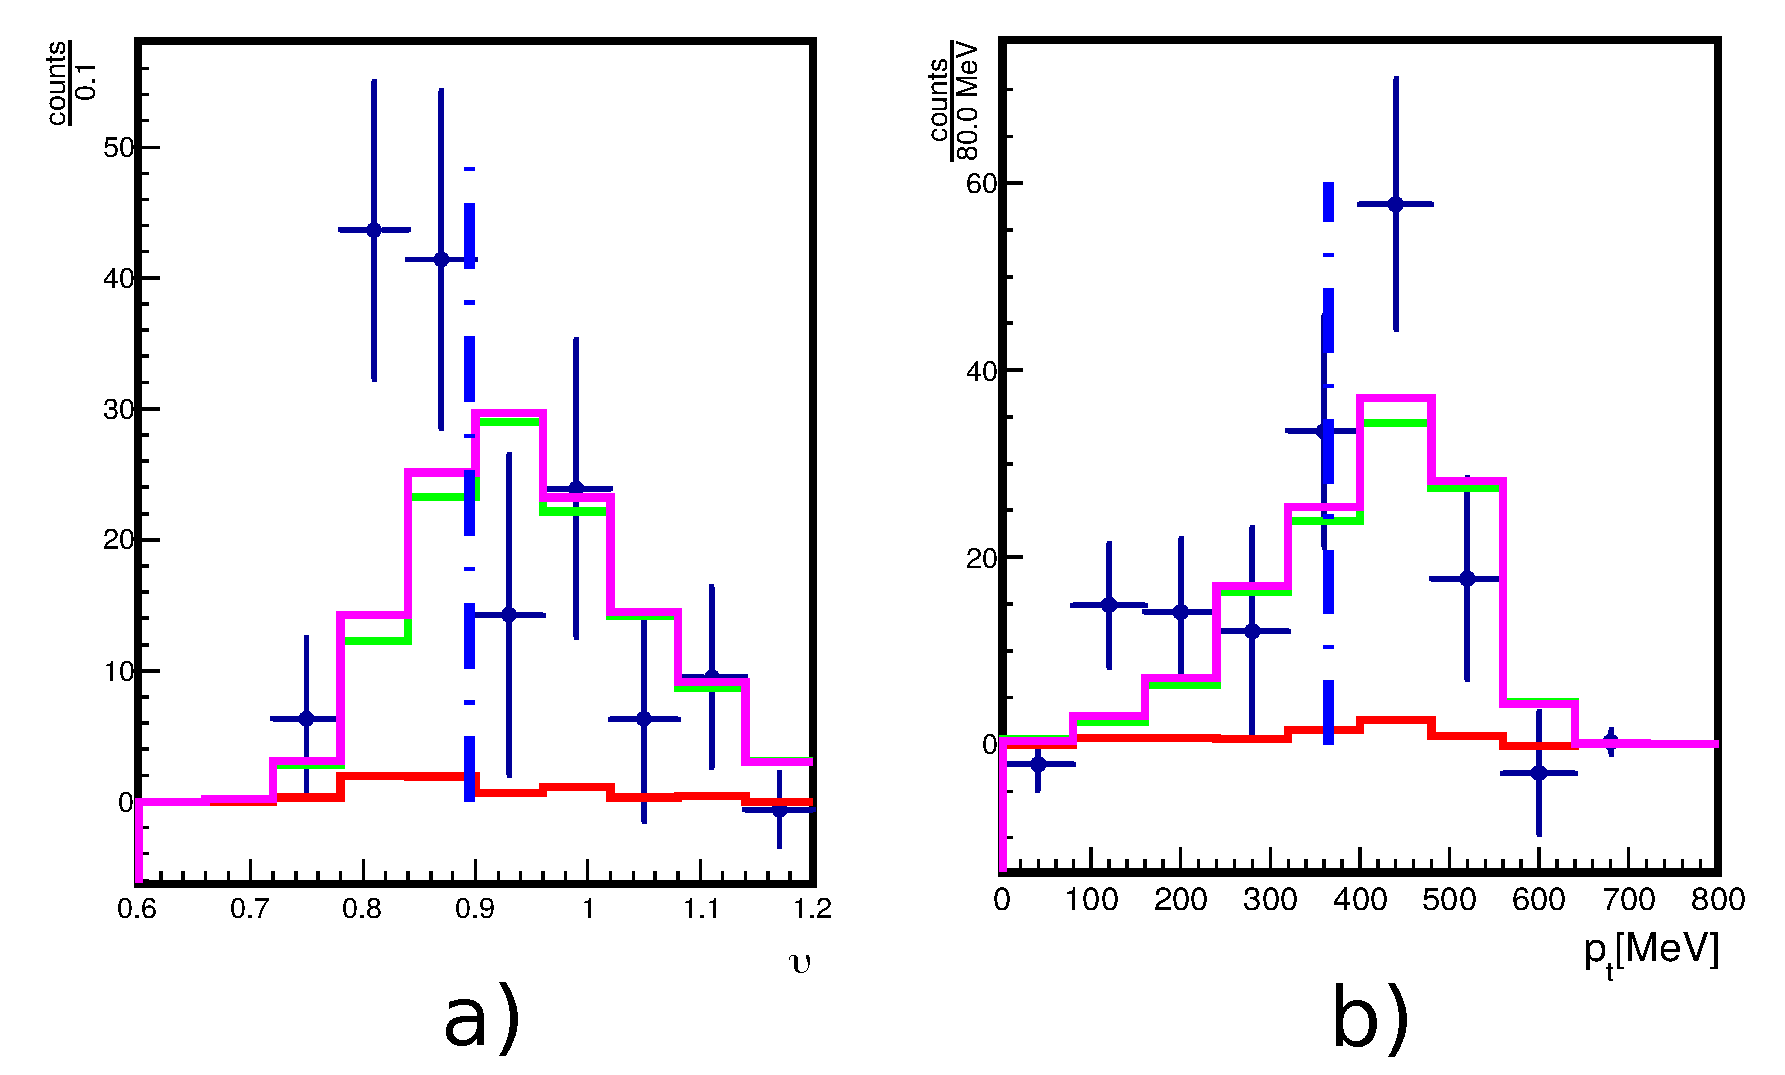
\includegraphics[width=0.9 \linewidth]{Chapter_analysis/WPt.eps}
  \includegraphics[width=0.9 \linewidth]{Data_pp/canvas_cPtW_thesis.eps}
  %\subfloat{\includegraphics[width=0.9 \linewidth]{Data_pp/}}
  \caption{Thw rapidity and $p_t$ spectrum for $\Ls$ events. Error bars denote statistical errors. The experimental data (blue points) is compared with the simulation (magenta line). A simulation is additionally decomposed into a signal channel (green line) and an combinatorial background (red line) contribution. Dashed vertical lines show a mean values for $p_t$ and w distribution. In both cases a vertical scale wase adjusted for an easy comparison with th esame spectra for pNb data (fig. \ref{fig:YPt_pNb}).}
  \label{fig:WPt}
\end{figure}



\subsection{Analysis of $\pip \pim$, $\Lz \pip$ and $\Lz \pim$ spectra}
In a model used for the signal simulation and \cs extraction, pions were emitted according to available phase-space. However results from an experiment pervormed by T. S. Mast at al. in Berkeley Laboratory in 1973 \cite{mast} allows for a partial wave analysis of $\Lz \pip \pim$ final state. The results suggests a leading role of $\Ss$ resonance in $\Ls$ decays. Also, some teoretical models suggest that the particle decays through $\Ss \pi$ state \cite{theory_Oset_photoproduction}. A possible $\Ss$ contribution would manifest by a distortion of a $\pip \pim$, $\p \pim \pip$ and $p \pim \pim$ spectra compared to direct production. Unfortunatelly, basing on statistics collected during the pp experiment it is hard to speculate about production mechanism and collected data do not allow for any final conclusions.  However the same spectra for pNb data \ref{chapter:analysis_pNb} brings a lot of interesting information. A $\pip \pim$\ref{fig:pip_pim}.  
\begin{figure}[h]
  \centering
  % 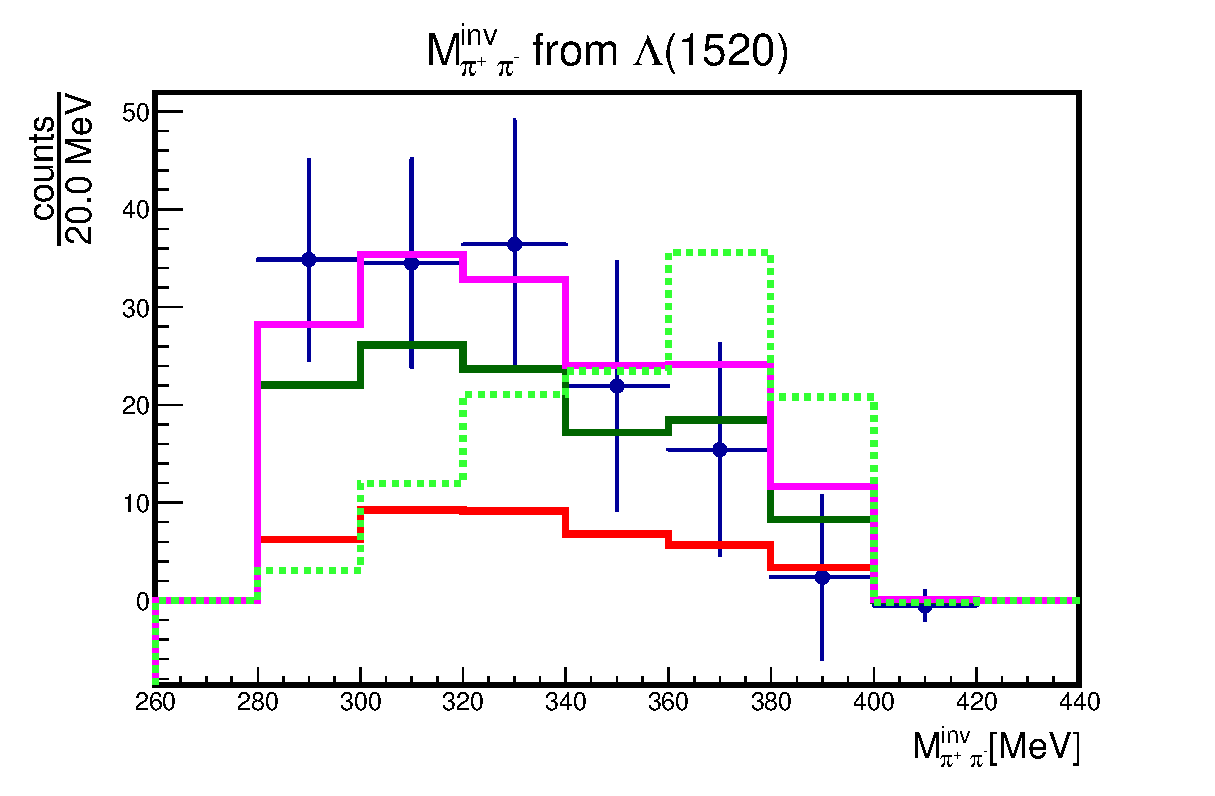
\includegraphics[width=0.9 \linewidth]{Chapter_analysis/PipPim.eps}
  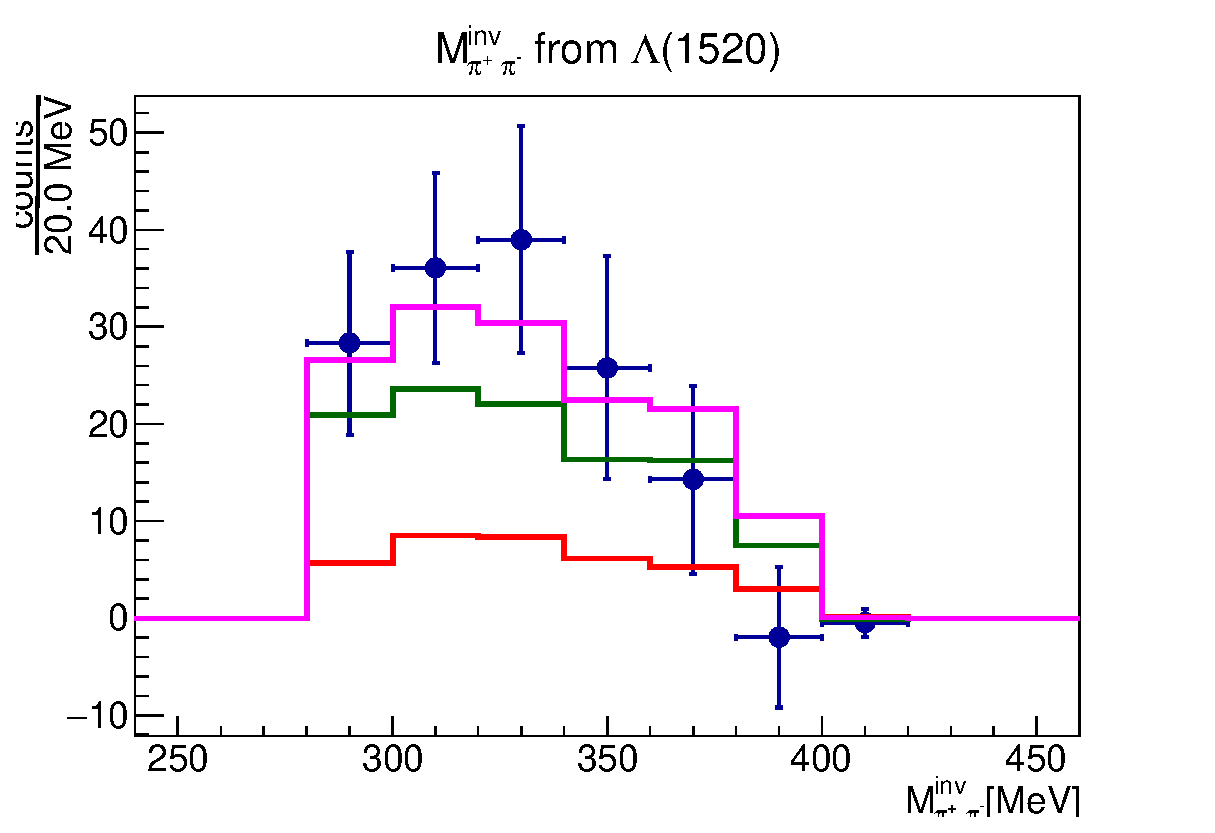
\includegraphics[width=0.9 \linewidth]{Data_pp/canvas_cClean_ren_PipPim.eps}
  \caption{The $\pip \pim$ from emitted from $\Ls$ events. The experimental data (blue points) is compared with signal (green line) and background (red line) simulation. A sum of simulated channels is shown by a magenta line. In the presented simulation a phase space pions distribution was used.  }
  \label{fig:pip_pim}
\end{figure}
\begin{figure}[bh]
  \centering
  % 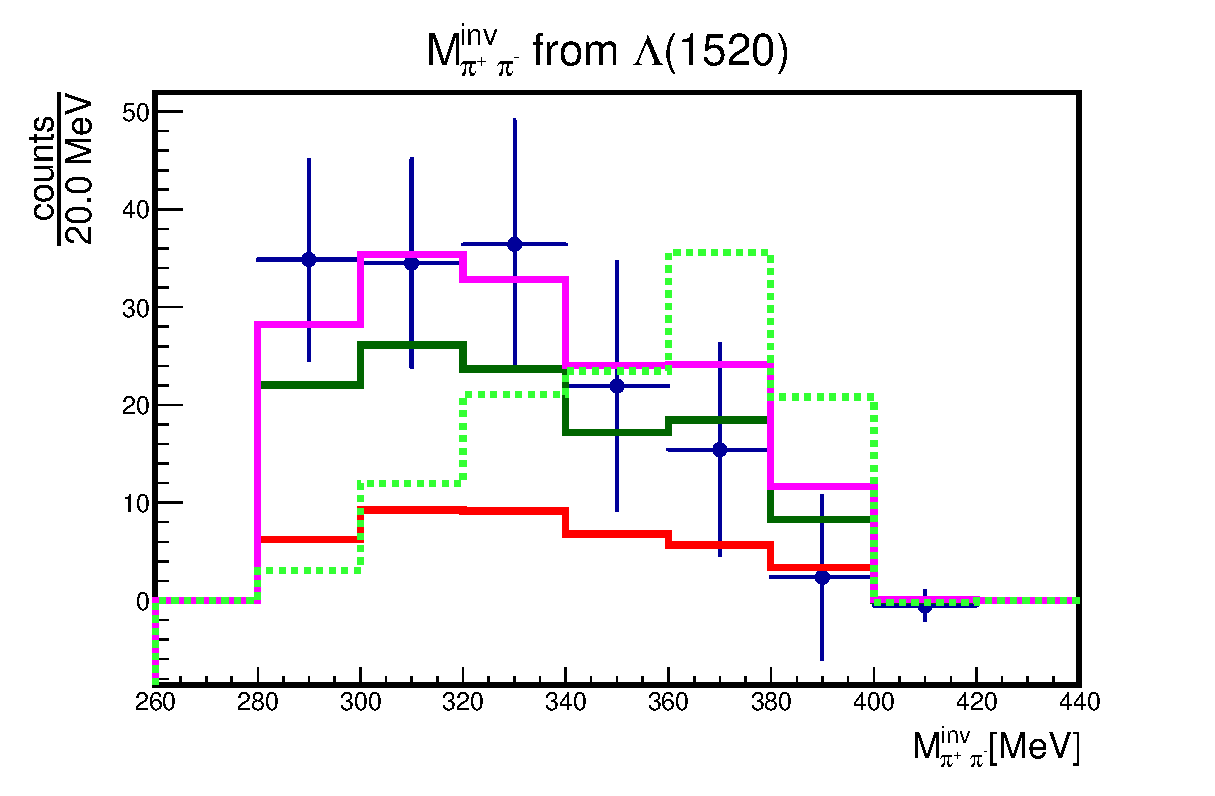
\includegraphics[width=0.9 \linewidth]{Chapter_analysis/PipPim.eps}
  %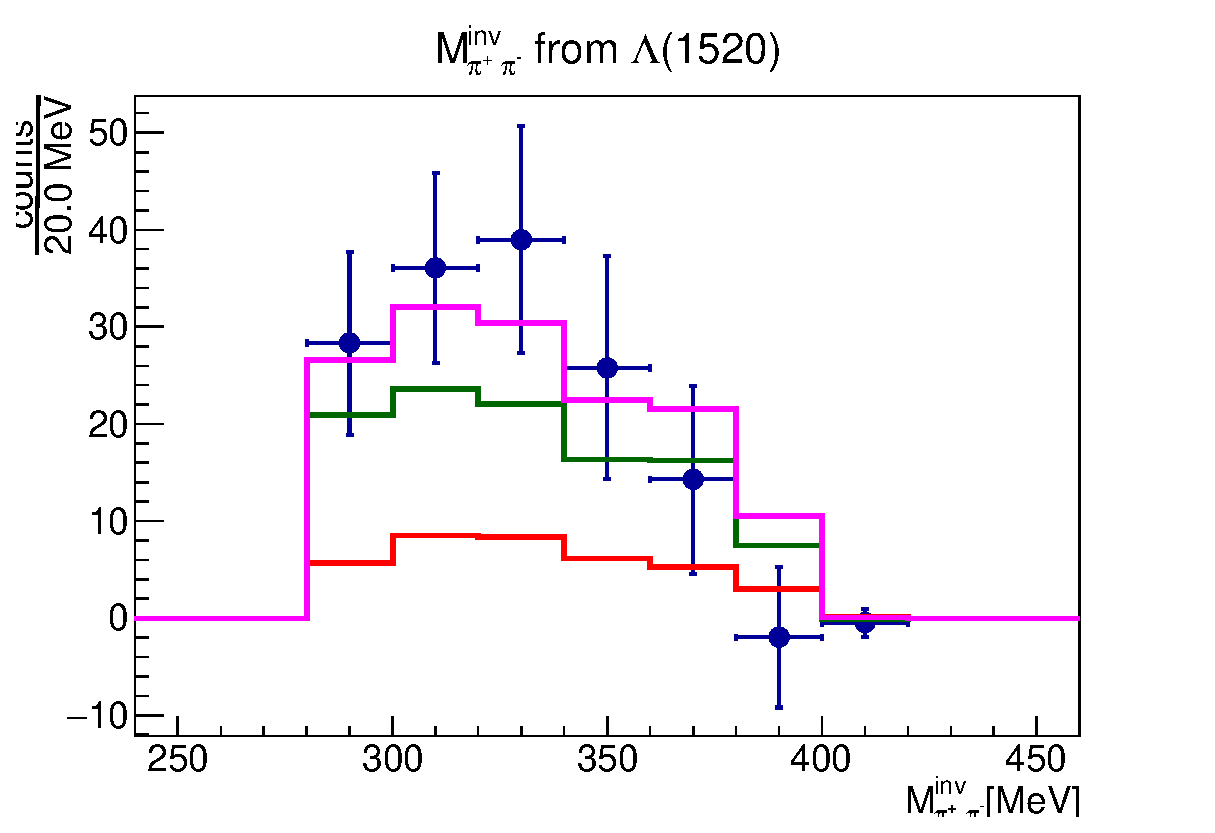
\includegraphics[width=0.9 \linewidth]{Data_pp/canvas_cClean_ren_PipPim.eps}
  \subfloat[ ]{\includegraphics[width=0.4 \linewidth]{Data_pp/canvas_cPPimPim_data_thesis.eps}}
 % \hfill
  \subfloat[ ]{\includegraphics[width=0.4 \linewidth]{Data_pp/canvas_cPPimPip_data_thesis.eps}}
 
  \caption{The $\pip \pim$ from emitted from $\Ls$ events. The experimental data (blue points) is compared with signal (green line) and background (red line) simulation. A sum of simulated channels is shown by a magenta line. In the presented simulation a phase space pions distribution was used.  }
  \label{fig:p_pip_pim}
\end{figure}




\section{Systematic error studies}
Through the entire studies the data is reduced from ??? events to ???. Each of the cuts used for analysis may be a potential source of systematic uncertainties. The most important cuts have been varied to estimate this effect. Tab \ref{tab:systematics} contains set of possible error sources. A size of the side-band regions seems to have minor impact for an systematic error. Similarly a fit range in which a signal and background were fitted does not influence the final result strongly. The most important factor comes from an opening angle between reconstructed and ideal $\Lz$ momentum.

\subsection{Uncorrelated error}
Varying a cut value allows to quantify a cut influence over the final result. However, statistical errors are still present in data and an effect of analysis with changed cuts also suffers from systematics. The situation is even more complicated, because a standard deviation for a counting process (a Poisson process) is equal $\sqrt{N}$ as long as events are independent. In case of the systematics studies different samples are strictly dependent. Loosening a cut someone can get a new, bigger, data sample, but almost all events in the sample belong to the original data set. Only few events are independent of the original data set. It is possible to estimate a statistical error connected with those "extra" events \cite{DA_CERN} using a formula
\begin{equation}
\sigma^2_{uncorr}=\abs{\sigma^2_A-\sigma^2_B}.    
\end{equation}


\begin{table}
\centering
  \caption{All analyzed sources of experimental unertentyties. Each value was obtained by varying the cuts around a central value. More details in text.}
  \label{tab:systematics}
  \begin{tabular}{rc}
    \hline
    A cut type & $\sigma$ [$\mu \barn$]\\
    \hline
    \hline
    Output of a neural network & 0.69\\
    A side-band range & 0.13\\
    A minimal distance between $\pim$ and $\p$&0.36\\
    An opening angle & 0.83\\
    Background channels \cs& \\
    \hline
    sum & \\
  \end{tabular}
\end{table}

\begin{figure}
  \centering
  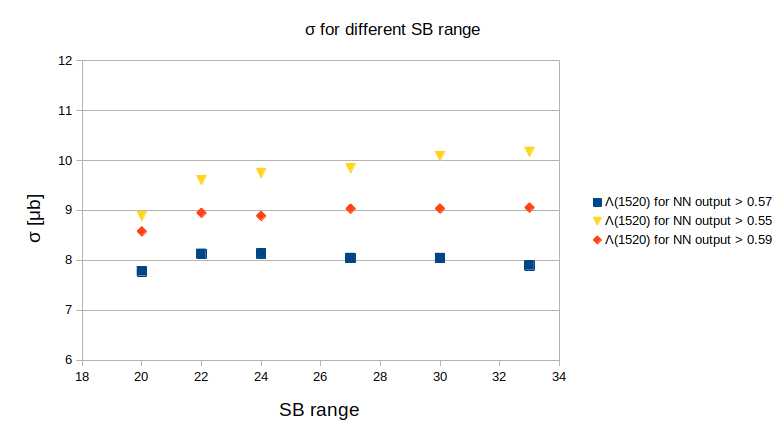
\includegraphics[width=0.9\linewidth]{Chapter_analysis/systematics_SB.png}
  \caption{The sistematic effect of different cut for neural network output. A broad range of cut was examinated, but values below 0.54 does not allow for a celan signal extraction. That causes systematical higher result.}
  \label{fig:systematics_NN}
\end{figure}
\begin{figure}
  \centering
  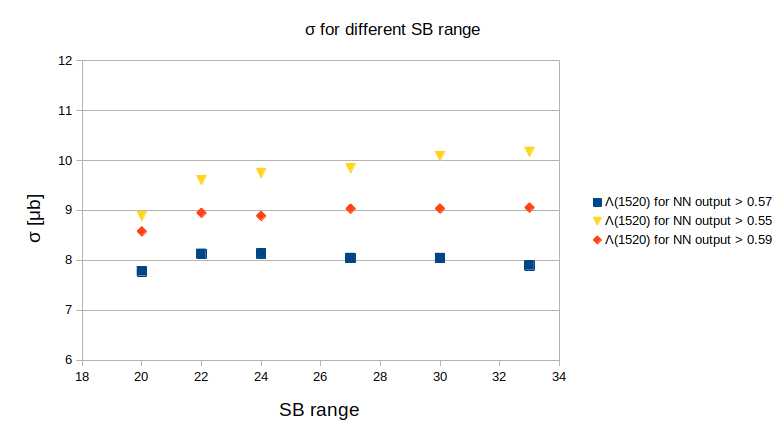
\includegraphics[width=0.9\linewidth]{Chapter_analysis/systematics_SB.png}
  \caption{The sistematic effect of different size of the side-band reagion. The central value (27) was set as the final one. An error bar for the central value shows statistic error associeted with limited statistics. For all other poins an uncorelated statistical error has been drawn. }
  \label{fig:systematics_SB}
\end{figure}
\begin{figure}
  \centering
  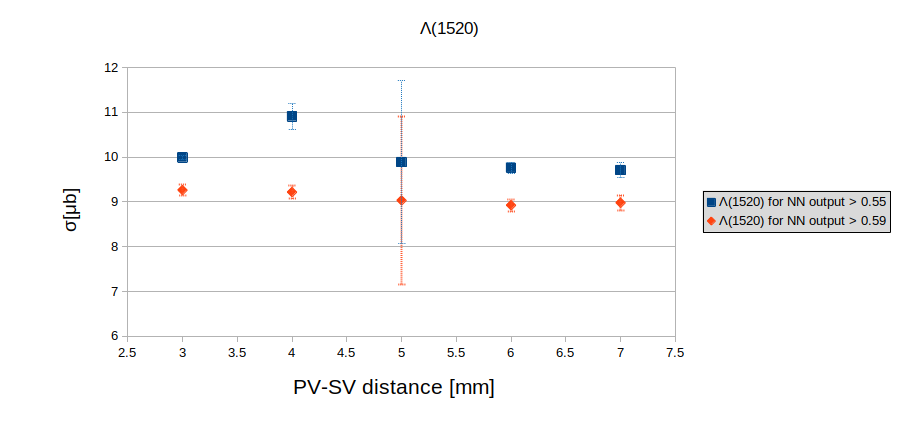
\includegraphics[width=0.9\linewidth]{Chapter_analysis/systematics_PV-SV.png}
  \caption{The sistematic effect of different minimal distance between primary and secondary vertex. The central value (5 mm) was set as the final one. An error bar for the central value shows statistic error associeted with limited statistics. For all other poins an uncorelated statistical error has been drawn. A behavour for two different cuts on NN network output was compared.}
  \label{fig:systematics_PV-SV}
\end{figure}
\begin{figure}
  \centering
  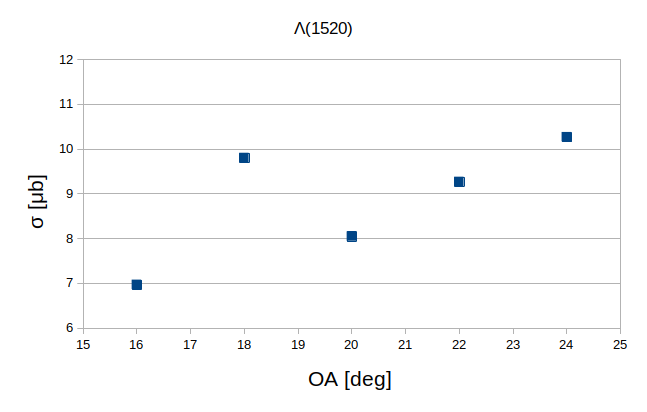
\includegraphics[width=0.9\linewidth]{Chapter_analysis/systematics_OA.png}
  \caption{The sistematic effect of different opening angle between $\Lz$ maomentum and streight line connecting primary and secondary vertex. The central value (<20 deg) was set as the final one. An error bar for the central value shows statistic error associeted with limited statistics. For all other poins an uncorelated statistical error has been drawn.}
  \label{fig:systematics_OA}
\end{figure}